\documentclass{article}
\usepackage{neurips_2026}
\usepackage[utf8]{inputenc}
\usepackage[T1]{fontenc}
\usepackage{hyperref}
\usepackage{url}
\usepackage{booktabs}
\usepackage{amsfonts,amsmath,amssymb}
\usepackage{nicefrac}
\usepackage{microtype}
\usepackage{graphicx}
\usepackage[table]{xcolor}
\graphicspath{{../figures/}}

\title{What Does a Tuned System's Benchmark Score Mean?\\Optimism After Prompt and Program Search, and How to Report It}

\author{Anonymous Author(s)}

\newcommand{\hatc}{\hat c}
\newcommand{\E}{\mathbb{E}}

\begin{document}
\maketitle

\begin{abstract}
A tuned LLM system is usually reported with its score on the same benchmark items that were used to search for its prompt or program. We ask how far such a score is from performance on fresh items, what drives the gap, whether it changes conclusions, and how to report more reliably. In a synthetic world with exact truth (203{,}400 search replicates) and on a real model and benchmark (Qwen2.5-1.5B-Instruct on MMLU-Pro, 300 candidate configurations replayed from cached outputs), the naive report is optimistic by up to 14.6 points (synthetic, 50 items, 200 candidates, no true differences) and 5.7 points on MMLU-Pro (100 search items, 300 candidates), roughly doubling the apparent gain over the baseline; the gap shrinks like $1/\sqrt n$, grows with the number of candidates and few-shot demonstrations drawn from the search set, and follows an extreme-value formula whose parameters we fit to each setting (a check of its form, not a held-out prediction). Naive reports declare a tuned system better than an untuned one in 97.6\% of synthetic replicates with no true gain; on MMLU-Pro such false-claim rates are not identifiable (the baseline is almost always truly worse), so decision errors rest on the synthetic world and a paired A-versus-B design on real outcomes, where reports rank systems by search effort. Hold-out and conditional/hybrid selection-aware intervals restore nominal coverage but cost items, width and power; empirical-Bayes disclosure fails. Results rest on one small model, template and ensemble configurations replayed from cached outputs on one fixed 2000-item pool (between-pool uncertainty is not estimated), and no live tool run.

\end{abstract}

\section{Introduction}
\label{sec:intro}
Automatic prompt and program optimisation has become routine: a tool such as DSPy~\citep{khattab2023dspy} or MIPRO~\citep{opsahlong2024mipro} searches instructions, demonstrations or multi-call pipelines on a set of benchmark items and the best configuration is reported with its score on benchmark items. When those items are the \emph{same} ones that drove the search, the number is a maximum over many noisy scores, not an unbiased estimate: it measures the winner's luck as well as the winner's quality. The consequence for the reader is unclear, because the size of the optimism, what governs it, and whether the comparisons built on such numbers (``our tuned system beats the baseline'', ``A beats B'') survive it are rarely examined for LLM systems.

We study this as a statistical question in a controlled setting. A search procedure with a budget evaluates $K$ configurations on $n$ items, returns $\hatc$, and the \emph{naive report} is the accuracy of $\hatc$ on those $n$ items; the target is its accuracy on fresh items. We ask (Q1) how large the gap is, what drives it, and whether it changes conclusions; and (Q2) whether more reliable reporting methods exist and how to test that they are.

\textbf{Contributions.} (1) A measurement of the optimism of the naive report in a synthetic world with exact truth (216 cells, 203{,}400 replicates) and on a real LLM and benchmark (Qwen2.5-1.5B-Instruct on 2000 MMLU-Pro questions, 300 prompt/ensemble configurations, 52 replay cells of 1000 replicates), with an extreme-value formula whose parameters are fitted in each setting (it checks the functional form; it is not a held-out prediction). (2) The decision-level consequence: naive reports declare a tuned system better than an untuned one when it is not, and rank two tuned systems by search effort and search-set size rather than by quality. These error rates rest on the synthetic world and, for real outcomes, on a paired A-versus-B design; the ``tuned beats baseline'' false-claim rate is not identifiable on MMLU-Pro, where the baseline is almost always truly worse. (3) A validation protocol with known truth and a real outcome matrix, applied to the reporting methods M0--M5 (naive, hold-out, cross-fitting, bootstrap optimism correction, simultaneous and conditional/hybrid selection-aware intervals, empirical-Bayes and Ladder-style disclosure), with an honest account of where each fails. (4) Scope: one small model on CPU, a prompt-format family rather than a search-heavy pipeline, emulated rather than live search (no DSPy/MIPRO run; the live tier and the 0.5B arm were not run), and a single fixed item pool whose between-pool variability is not estimated (Sec.~\ref{sec:discussion}); our real-LLM claims are limited accordingly.

\section{Related Work}
\label{sec:related}
\textbf{Prompt and program optimisation.} DSPy compiles declarative LM programs by searching instructions and demonstrations against a metric on a training set~\citep{khattab2023dspy}; MIPRO jointly optimises instructions and demonstrations of multi-stage programs~\citep{opsahlong2024mipro}; best-arm-identification formulations select prompts under a limited evaluation budget~\citep{shi2024bai}. These works report the score of the selected configuration on held-out data of a given size; we ask what such a number means when the same items drive selection and scoring, and how it depends on the search budget.

\textbf{Evaluation variability of prompts.} Prompt format alone changes accuracy substantially~\citep{sclar2024formatting}, and prompt-performance distributions can be estimated from few evaluations~\citep{polo2024multiprompt}. This supplies the between-configuration spread that, in our analysis, drives the selection effect.

\textbf{Adaptive data analysis and test-set reuse.} Reusing a holdout adaptively invalidates naive estimates~\citep{dwork2015adaptive}; the Ladder reports thresholded leaderboard scores to limit overfitting~\citep{blum2015ladder}. Empirical studies of test-set reuse find smaller drift than worst-case bounds suggest~\citep{recht2018cifar,mania2019similarity}. We study the same phenomenon for automatic prompt/program search with an explicit selection step, and compare the Ladder-style report as a baseline.

\textbf{Selection-aware inference.} Winner's-curse corrections and conditional/hybrid intervals for selected targets~\citep{andrews2024winners}, simultaneous inference over selected models~\citep{berk2013valid}, Gaussian multiplier-bootstrap bounds for maxima~\citep{chernozhukov2013gaussian}, and the target-of-estimation analysis of cross-validation~\citep{bates2024cv} provide the tools we adapt to reporting a tuned system's score.

\section{Setting, Estimands and Reporting Methods}
\label{sec:method}
% DRAFT: definitions follow the study plan (story-repo plan/study-plan.md); to be reconciled with the implemented estimators in experiment-repo before release.
\textbf{Setting.} A system has a configuration space $\mathcal C$ (an instruction/prompt, or a multi-call program with demonstrations). A search procedure $S$ with budget $B$ evaluates configurations on a \emph{search set} $D$ of $n$ benchmark items and returns a configuration $\hatc$. Let $\theta(c)$ be the accuracy of $c$ on the item population (fresh items) and $R(c;D)$ its accuracy on $D$. The \emph{naive report} is $R(\hatc;D)$.

\textbf{Estimands.} The optimism is $\Delta=R(\hatc;D)-\theta(\hatc)$; we study $\E[\Delta]$, its quantiles, and the bias of the naive report for $\theta(\hatc)$. Reporting methods are judged on bias, RMSE, coverage of $\theta(\hatc)$ at nominal 95\%, interval width, data cost, and the error rates of claims made from them (``tuned beats baseline by margin $m$'', ``A beats B'').

\textbf{Reporting methods.} M0 naive; M1 holdout (search on $D_s$, report on disjoint $D_r$); M2 cross-fitting (repeat search per fold, pooled out-of-fold score; estimates the expected fresh accuracy of the \emph{procedure}, not of one $\hatc$); M3 bootstrap optimism correction; M4 selection-aware inference (simultaneous multiplier-bootstrap bound over all evaluated configurations; winner's-curse-adjusted intervals); M5 disclosure of the searched-candidate score distribution with $K$ and $n$, and a Ladder-style thresholded report.

\textbf{Extreme-value approximation.} For exhaustive search over $K$ candidates with per-item outcome SD $\sigma$ (candidate accuracy $\theta_0$, $\sigma^2=\theta_0(1-\theta_0)$), binary item-outcome correlation $r$ between candidates and true-accuracy spread $\tau_p$ (probability scale), $s^2=\sigma^2(1-r)/n$ is the candidate-specific part of the sampling variance of a search-set score, and we use
\begin{equation}
\E[\Delta]\;\approx\;\frac{s^2\,g(K)}{\sqrt{\tau_p^2+s^2}},\qquad g(K)=\E\max_{k\le K}Z_k,\; Z_k\stackrel{iid}{\sim}\mathcal N(0,1),
\end{equation}
the winner's-curse of the maximum of $K$ noisy scores around a true spread $\tau_p$; at $\tau_p=0$ it reduces to $s\,g(K)$. It is a heuristic (Gaussian, independent-noise approximation of correlated binary scores), checked against simulation and the real matrix rather than derived with error bounds.

\section{Experiments}
\label{sec:experiments}
Every number below is read from files in \texttt{results/} produced by the shipped code (script map in \texttt{figures/SCRIPTS.md}; commands in \texttt{REPRODUCE.md}). Intervals over replicates are mean$\pm1.96\,$SE; coverage and decision rates carry Wilson 95\% intervals (T0); on the real matrix (T1) replicates share one item pool, so T1 intervals are delete-a-block.

\subsection{Synthetic world with exact truth (T0)}
\textbf{Design.} A latent-probit world: each configuration $c$ has a true accuracy $\theta_c=\Phi(a+\delta_c)$ with spread $\tau$ (SD of $\delta_c$ on the probit scale; $\tau=0$ means all configurations are equal), item difficulty is shared across configurations with latent correlation $\rho$ of configuration$\times$item effects, and outcomes are Bernoulli. Because $\theta(\hatc)$ is known exactly, bias and coverage are measured without noise on the truth. The grid covers $n\in\{50,\dots,2000\}$, $K\in\{2,\dots,200\}$ candidates, $\tau\in\{0,.05,.1,.2\}$, $\rho$, baseline accuracy, three search procedures (exhaustive, successive halving, greedy coordinate edit) and few-shot demonstrations drawn from $D$: 216 cells and 203{,}400 replicates (300--1000 per cell). The reference world is $\rho=0.6$, baseline accuracy 0.3, exhaustive search; the headline cells have 1000 replicates.

\textbf{How large is the gap, and what drives it?} (Fig.~\ref{fig:A}.) The naive report is optimistic in every cell with $K>1$ configurations compared. With $\tau=0$ (nothing to find) the mean optimism is 14.6 [14.2, 14.9] accuracy points at $n=50$, $K=200$, 4.5 [4.4, 4.6] at $n=500$ and 2.2 [2.1, 2.2] at $n=2000$; at $n=200$ it is 2.9 [2.8, 3.1] for $K=5$ and 5.7 [5.5, 5.8] for $K=50$. It shrinks roughly as $1/\sqrt n$ and grows with $K$ like the expected maximum of $K$ noise terms; the closed-form extreme-value approximation $s^2g(K)/\sqrt{\tau_p^2+s^2}$ (Sec.~\ref{sec:method}) is within 0.84 points of the measurement over all 128 reference cells (mean theory$-$measurement $-0.13$ points). A larger true spread $\tau$ \emph{reduces} the optimism (the search finds real signal), but at $K=200$, $n=50$ it remains 9.0 points at $\tau=0.2$. Fig.~\ref{fig:B}: search procedures that evaluate fewer candidates on all items (halving, greedy) are less optimistic than exhaustive search (at $n=200$, $K=50$, $\tau=0$: 5.0 and 4.3 vs.\ 5.7 points), high correlation between configurations' item outcomes reduces it (7.0 points at $\rho=0.2$, 3.9 at $\rho=0.9$), baseline accuracy matters little (4.6, 5.7, 6.2 points at 0.15, 0.30, 0.50), and drawing few-shot demonstrations from $D$ adds optimism (at $K=24$, $n=50$, $\tau=0$: 13.1 vs.\ 10.0 points; at $n=200$: 5.7 vs.\ 4.9).

\begin{figure}[t]
\centering
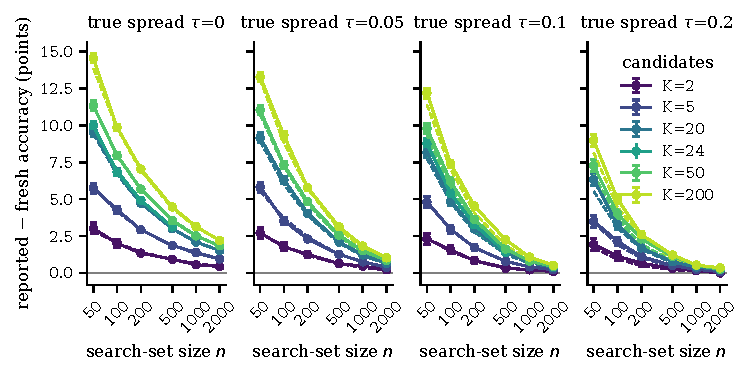
\includegraphics[width=\linewidth]{fig_a_optimism.pdf}
\caption{\textbf{Optimism of the naive report in the synthetic world (T0).} Reported minus fresh-item accuracy of the selected configuration against search-set size $n$, for $K$ candidates searched exhaustively, one panel per true spread $\tau$. Points: mean over 1000 replicates per cell, bars: 95\% CI; dashed: extreme-value prediction. Reference world $\rho=0.6$, baseline accuracy 0.3.}
\label{fig:A}
\end{figure}
\begin{figure}[t]
\centering
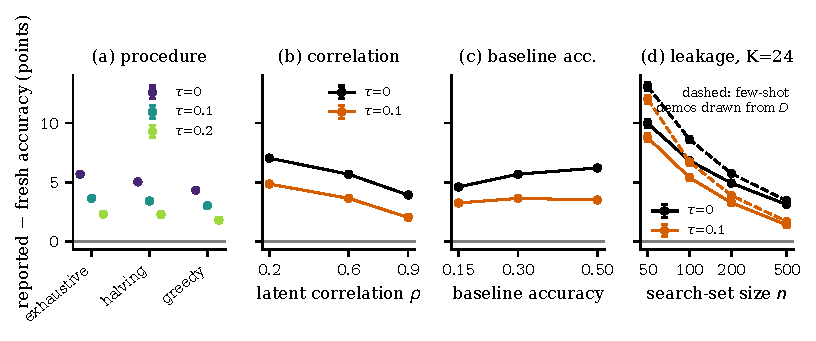
\includegraphics[width=\linewidth]{fig_b_factors.pdf}
\caption{\textbf{Other drivers of optimism (T0).} Same quantity; $n=200$, $K=50$ unless stated. (a) search procedure, (b) correlation $\rho$ between configurations' item outcomes, (c) baseline accuracy, (d) few-shot demonstrations drawn from $D$ (dashed) or not, $K=24$. 1000 replicates per point.}
\label{fig:B}
\end{figure}

\textbf{Does it change conclusions?} (Tables~\ref{tab:D},~\ref{tab:E}.) Take the claim ``tuned beats the untuned baseline by more than $m=2$ points'' with $K=200$, $n=100$. When the truth is $\tau=0$ (no gain), the naive point comparison claims it 97.6 [96.5, 98.4]\% of the time. Comparing two tuned systems on reported scores, the system searched over $K=200$ candidates is declared better than one searched over $K=5$ in 86.7 [84.5, 88.7]\% of replicates although they are equal, and a system tuned on $n=50$ items beats one tuned on $n=500$ in 93.2 [91.5, 94.6]\% of replicates ($K=50$). The reported ranking thus tracks search effort and set size rather than quality.

\subsection{Reporting methods: calibration and decisions (T0)}
\textbf{Targets and metrics.} Each method reports an estimate and, where available, a nominal 95\% interval for $\theta(\hatc)$ (M2: for the expected fresh accuracy of the fold-selected configurations). We measure bias, RMSE, coverage, width and the number of items consumed (Table~\ref{tab:C}, Fig.~\ref{fig:C}).

\begin{figure}[t]
\centering
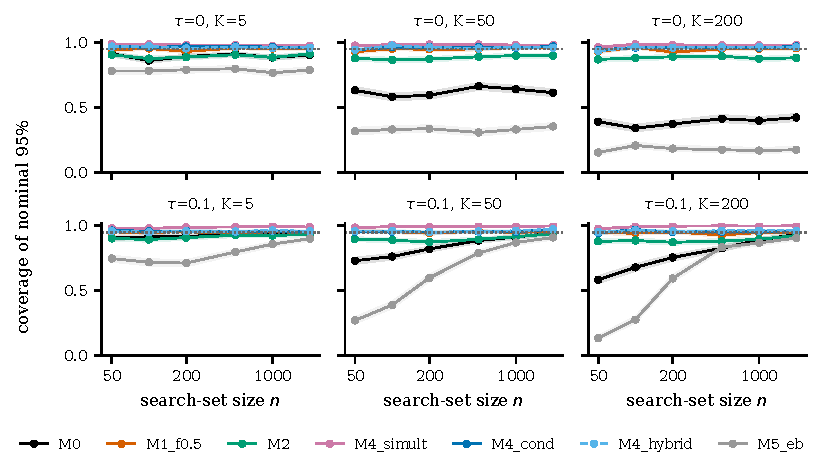
\includegraphics[width=\linewidth]{fig_c_coverage.pdf}
\caption{\textbf{Coverage of nominal-95\% intervals (T0).} Wilson 95\% bands over 1000 replicates; dotted: 0.95. M0: same-set interval; M1\_f0.5: hold-out with half of $D$ for selection; M2: 5-fold cross-fitting; M4\_simult: simultaneous max-type bound; M4\_cond, M4\_hybrid: conditional/hybrid selection-aware intervals; M5\_eb: empirical Bayes from disclosed scores.}
\label{fig:C}
\end{figure}

\begin{table}[t]
\caption{\textbf{Calibration of reporting methods (T0), $K=200$, $n=100$, 1000 replicates per cell} ($n=500$ and the other methods in the appendix, Table~\ref{tab:Cfull}). Bias and RMSE in accuracy points; coverage with Wilson 95\% interval; width in points; items used for the report. Ladder/optimism-corrected point reports have no interval and appear in the appendix.}
\label{tab:C}
\centering\scriptsize
\resizebox{\linewidth}{!}{\begin{tabular}{llrrrrrr}
\toprule
$\tau$ & $n$ & method & bias (pts) & RMSE (pts) & coverage [Wilson 95\%] & width (pts) & items for report \\
\midrule
0 & 100 & M0 & +9.85 $\pm$ 0.21 & 10.40 & 0.341 [0.312, 0.371] & 18.9 & 100 \\
0 & 100 & M1\_f0.5 & -0.08 $\pm$ 0.40 & 6.38 & 0.964 [0.951, 0.974] & 24.6 & 50 \\
0 & 100 & M2 & -0.03 $\pm$ 0.34 & 5.49 & 0.880 [0.858, 0.899] & 17.7 & 100 \\
0 & 100 & M4\_simult & +9.85 $\pm$ 0.21 & 10.40 & 0.986 [0.977, 0.992] & 34.2 & 100 \\
0 & 100 & M4\_cond & -3.99 $\pm$ 1.86 & 30.22 & 0.961 [0.947, 0.971] & 45.8 & 100 \\
0 & 100 & M4\_hybrid & +2.61 $\pm$ 0.46 & 7.94 & 0.964 [0.951, 0.974] & 27.3 & 100 \\
0 & 100 & M5\_eb & -0.09 $\pm$ 0.17 & 2.81 & 0.208 [0.184, 0.234] & 1.3 & 100 \\
0 & 100 & M5\_ladder & -1.17 $\pm$ 0.63 & 10.26 & -- & -- & 100 \\
\midrule
0.1 & 100 & M0 & +7.40 $\pm$ 0.25 & 8.40 & 0.680 [0.650, 0.708] & 19.1 & 100 \\
0.1 & 100 & M1\_f0.5 & -0.29 $\pm$ 0.42 & 6.73 & 0.943 [0.927, 0.956] & 25.4 & 50 \\
0.1 & 100 & M2 & -0.35 $\pm$ 0.37 & 5.90 & 0.886 [0.865, 0.904] & 18.4 & 100 \\
0.1 & 100 & M4\_simult & +7.40 $\pm$ 0.25 & 8.40 & 0.993 [0.986, 0.997] & 34.6 & 100 \\
0.1 & 100 & M4\_cond & -3.21 $\pm$ 1.44 & 23.42 & 0.970 [0.957, 0.979] & 41.5 & 100 \\
0.1 & 100 & M4\_hybrid & +1.34 $\pm$ 0.46 & 7.52 & 0.964 [0.951, 0.974] & 27.5 & 100 \\
0.1 & 100 & M5\_eb & -4.67 $\pm$ 0.24 & 6.05 & 0.278 [0.251, 0.307] & 5.3 & 100 \\
0.1 & 100 & M5\_ladder & -1.48 $\pm$ 0.63 & 10.20 & -- & -- & 100 \\
\bottomrule
\end{tabular}
}
\end{table}

\textbf{Findings (T0, $K=200$, $\tau=0$, $n=100$; Table~\ref{tab:C}).} The naive interval covers $\theta(\hatc)$ in only 34.1 [31.2, 37.1]\% of replicates (bias $+9.85\pm0.21$ points); even at $n=500$ coverage is 41.4\%, and at $\tau=0.1$ it is 68.0\% and 82.7\% at $n=100$ and $500$. (i) \emph{Hold-out} (M1) is unbiased and covers at the nominal level (0.96 for all three split fractions), but it pays in items and width: 19.7 to 37.3 points wide at $n=100$ and, with half of $D$ held out, RMSE 6.4 vs.\ 10.4 points for M0. (ii) \emph{Cross-fitting} (M2) is unbiased for the expected fresh accuracy of the procedure's selections but its interval undercovers (0.88 [0.86, 0.90]; 0.86--0.95 over the 128 reference cells), because fold scores are dependent. (iii) \emph{Selection-aware inference} (M4): the simultaneous bound covers (0.986) but is as biased as M0 and wide (34.2 points); the conditional (0.961) and hybrid (0.964, width 27.3 points) intervals reach nominal coverage (0.94--0.98 over the 128 reference cells, as for M1\_f0.5 at 0.92--0.97), but the conditional point estimate is heavy-tailed (RMSE 30 points at $n=100$) so only its interval is usable, and hybrid has bias $+2.6$ points. (iv) Bootstrap optimism correction (M3) removes only part of the bias ($+1.9$ points for $n=200$; $+2.5$ for the .632 variant, vs.\ $+7.0$ for M0; appendix). (v) The empirical-Bayes interval from the disclosed scores (M5\_eb) fails: coverage 0.21 at $\tau=0$, $K=200$, $n=100$, and 0.09--0.93 across the 128 reference cells (Fig.~\ref{fig:C}), since candidates share items; we report it as a negative result. The Ladder-style report has no interval; its point report is $-1.2\pm0.6$ points biased with step $n^{-1/3}$ but $+8.2\pm0.3$ with the $0.5/\sqrt n$ step, i.e.\ its calibration depends on a free step size.

\begin{table}[t]
\caption{\textbf{False-claim rate and power of ``tuned beats baseline by $>2$ points'' (\%, Wilson 95\%), $K=200$, $n=100$ (T0).} ``point'': estimate difference exceeds $m$; ``lower bound'': the method's 95\% lower bound exceeds the baseline's estimate $+m$. At $\tau=0$ the true gain is 0. At $\tau=0.1$, 162 false-claim and 608 power replicates (per-cell counts in \texttt{tables/table\_d\_all\_cells.csv}).}
\label{tab:D}
\centering\scriptsize
\resizebox{\linewidth}{!}{\input{../tables/table_d_decisions.tex}}
\end{table}

\textbf{Decisions (Table~\ref{tab:D}).} Naive reports make a false improvement claim in 97.6\% of replicates when there is no improvement; using the naive lower bound this is still 38.4 [35.4, 41.5]\%. Hold-out, cross-fitting and the selection-aware lower bounds bring the false-claim rate to 0.5--4.1\% with a lower-bound rule, but at this sample size the price is power: at $\tau=0.1$ the power to detect a true gain of $\geq 2$ points falls from 73.7 [70.6, 76.6]\% (naive lower bound, which is not valid) to 10.8--27.4\% (valid rules). The point-comparison rule has a high false-claim rate even for unbiased methods (32--43\% for M1/M2) because the difference of two noisy scores exceeds $m=2$ points by chance; \emph{unbiasedness does not by itself license a claim}.
\subsection{Real LLM on real MMLU-Pro (T1)}
\label{sec:t1}
\textbf{Design.} The system is Qwen2.5-1.5B-Instruct~\citep{qwen2024qwen25} (Q8\_0 GGUF, llama.cpp, CPU; Apache-2.0) answering MMLU-Pro~\citep{wang2024mmlupro} (pinned revision, MIT license, 10 options) by reading out the log-probabilities of the ten option letters. The configuration family has 24 base prompts (4 instruction styles $\times$ 2 answer cues $\times$ \{0-shot, two 3-shot demonstration sets from the validation split\}) plus the 276 two-prompt logit-average ensembles of them as a pipeline-like extension: $K_{\max}=300$ candidates. All 300 are scored once on a fixed pool of 2000 randomly drawn test questions and the per-item outcomes are cached; a search is then \emph{replayed}: draw a search set $D$ of $n$ pool items, let the procedure choose $\hatc$ among $K$ candidates (the baseline prompt plus $K-1$ random ones; $K=24$ is the base family), and score $\hatc$ on the remaining pool items minus a left-out block (1300--1750 fresh items, binomial SE $\approx$1.1--1.3 points, independent of the search). The pool accuracies of the 24 base prompts range from 20.5\% to 29.2\% and the best of all 300 is 30.1\%; the between-candidate spread is small ($\tau\approx0.017$--$0.024$ on the probability scale) and candidates are strongly correlated (binary item correlation 0.57--0.68). The baseline prompt has 22.7\%. 52 replay cells with 1000 replicates each; because replicates share the fixed pool, every uncertainty in this subsection is $\pm1.96\times$ a delete-a-block SE (10 blocks of replicates) rather than a replicate SE or Wilson interval; it reflects the variation over search sets given the pool, not the uncertainty about the pool itself, which we do not estimate.

\textbf{Gap.} (Fig.~\ref{fig:A1}.) The naive report is optimistic here too. For $K=300$ and $n=100$ the selected configuration is reported at 33.7\% and scores 28.0\% on fresh items: a 5.7-point gap (block SE 0.11). Against the baseline's 22.7\%, the reported improvement is 11.0 points while the real one is 5.3: about twice as large. The gap is 8.7 points at $n=50$ and 1.9 at $n=500$ ($K=300$), and 4.6 points for the 24 base prompts alone ($n=100$). It grows with $K$ and falls with $n$ like the extreme-value formula evaluated with the matrix's own $(\sigma,r,\tau)$, which is within 0.51 points of every one of the 35 exhaustive cells (mean difference $-0.04$ points), although 13 of the 35 differ by more than 1.96 block SE, mostly at small $K$ and $n=50$ where it over-predicts (e.g.\ $K=2$, $n=50$: 1.80 predicted, 1.29 observed). The parameters are estimated from the same matrix, so this checks the functional form, not a held-out prediction. The synthetic grid of T0 gives a larger gap than the real one in 28 of its 30 nearest cells (median ratio 1.6; its correlation grid does not contain the matrix's), so we treat T0 as a model of the mechanism, not a calibrated replica (Fig.~\ref{fig:T1check}, appendix). Halving and greedy search are mildly less optimistic than exhaustive search (4.0 and 4.1 vs.\ 4.5 points at $n=100$, $K=24$; 5.2 vs.\ 5.7 at $K=300$). The gap is present in every one of the 14 MMLU-Pro subjects (3.3 to 7.0 points at $n=100$, $K=24$; Fig.~\ref{fig:T1subj}, appendix).

\textbf{Reporting methods and decisions.} (Table~\ref{tab:G}.) The naive interval covers $\theta(\hatc)$ in 77.1 $\pm$ 3.2\% ($n=100$) and 80.6 $\pm$ 2.2\% ($n=500$; $\pm1.96$ block SE) of replicates at $K=300$ and is biased by $+5.7$ and $+1.9$ points. Hold-out (M1, 0.95/0.94 at half split), the hybrid conditional interval (0.953/0.935) and cross-fitting (0.92/0.88) are close to nominal and unbiased; the conditional interval is nominal but its point estimate is heavy-tailed (RMSE 20.8 points at $n=100$); the simultaneous bound is conservative (0.988) and as biased as M0; the empirical-Bayes interval again fails (0.11/0.22). Bootstrap optimism correction removes most but not all of the bias ($+1.8$ points at $n=100$, $K=300$, vs.\ $+5.7$ for M0; appendix). Because the 276 ensembles are not independent systems and the candidates differ little, "tuned beats baseline" is almost always true here, so false-claim rates are not identifiable from these cells; we use a paired design instead (Table~\ref{tab:H}): two systems tuned with $K_A=75$ and $K_B=5$ candidates on the same $n=100$ items, where the true difference is on average 0.5 points and A is truly better in only 61.7\% of the replicates. Naive reports declare A better in 90.3\% of replicates (the reported difference is $+3.0$ points against a true $+0.5$); among the 383 replicates in which A is not truly better, 87.5\% still call it better with M0, versus 43--56\% for hold-out, cross-fitting and the selection-aware point rules. With a rule that requires A's 95\% lower bound to exceed B's estimate the false-winner rate is 0\% for M0 and the simultaneous bound and 3.1--3.4\% for hold-out, cross-fitting and the conditional/hybrid intervals, but those rules detect a truly better A in only 7--9\% of replicates (M0: 1.8\%); the equal-$K$ pairs have no true difference, and every report order there is a coin flip (flip rates near 0.5 by construction).

\begin{figure}[t]
\centering
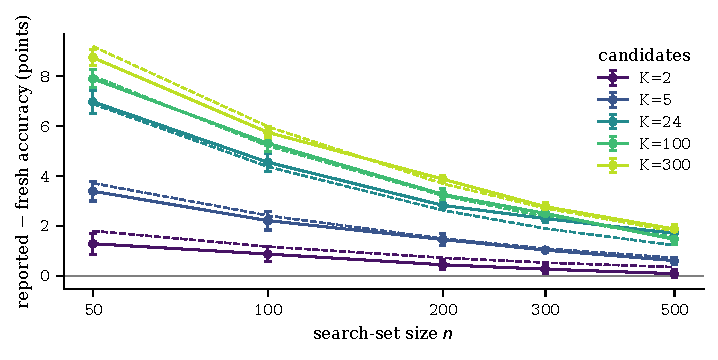
\includegraphics[width=\linewidth]{fig_a_t1.pdf}
\caption{\textbf{Optimism of the naive report on the real outcome matrix (T1).} Reported minus fresh-item accuracy of the selected configuration against $n$, for $K$ candidates searched exhaustively (Qwen2.5-1.5B-Instruct, MMLU-Pro; 1000 replicates per cell). Bars: mean $\pm1.96\times$ delete-a-block SE (replicates share one 2000-item pool, so the replicate SE is too small); dashed: the closed form fed with the matrix's own $(\sigma,r,\tau)$.}
\label{fig:A1}
\end{figure}

\begin{table}[t]
\caption{\textbf{Calibration of reporting methods on the real matrix (T1), $K=300$, $n=100$, 1000 replicates} ($n=500$ in the appendix). Bias and RMSE in points against each method's own target; coverage $\pm1.96$ block SE; median width (points); items used for the report.}
\label{tab:G}
\centering\scriptsize
\resizebox{\linewidth}{!}{\input{../tables/table_g_main.tex}}
\end{table}

\begin{table}[t]
\caption{\textbf{Ranking two tuned systems on the same search set (T1).} A and B are tuned exhaustively from disjoint candidate subsets of $K_A$ and $K_B$ configurations; 1000 replicates per cell, $\pm1.96$ block SE. Flip: the reported order differs from the true order (a tie counts as a flip). The 75 vs.\ 5 pair has the largest search-effort contrast; the equal-$K$ pairs are controls with no true difference.}
\label{tab:H}
\centering\scriptsize
\resizebox{\linewidth}{!}{\input{../tables/table_h_t1_pairs.tex}}
\end{table}


\section{Discussion and Limitations}
\label{sec:discussion}
\textbf{What to report.} The evidence supports a conditional answer. The naive report of a searched system is biased upward whenever more than one configuration is compared on the same items; the bias is of the order of the true differences between configurations when $n$ is a few hundred and $K$ is large, so reported improvements of a few points are not interpretable without $n$ and $K$. Reporting the score of $\hatc$ on items not used for the search (M1) removes the bias at the price of items; a conditional/hybrid selection-aware interval (M4) gives nominal coverage for exhaustive search without extra items but needs the full score table and, in our runs, is wide; cross-fitting (M2) estimates the performance of the procedure, with mildly undercovering intervals. At minimum a report should state $K$, $n$ and the search procedure, and avoid comparing systems tuned with different $K$ or $n$ on reported scores. Methods that look attractive can fail: empirical-Bayes shrinkage of disclosed scores assumes independent noise, and the Ladder-style report depends on a free step size.

\textbf{Limitations.} (i) The real-LLM evidence is one 1.5B-parameter model on a pool of 2000 MMLU-Pro questions on CPU; no larger model, second benchmark or second task was run, so we make no statement about frontier systems. (ii) The candidates are prompt formats and two-prompt ensembles; their true spread is small and they are correlated, which is a low-signal regime; real prompt/program search with instruction proposals may have larger spread and adaptive proposals that our three procedures (exhaustive, halving, greedy) only approximate. (iii) T1 is a replay on cached outcomes, \emph{not} a live run of DSPy/MIPRO; the live-tool tier of our plan was not done. (iv) The pool is fixed, and the uncertainty in T1 is over search sets given the pool; between-pool uncertainty was not estimated; the block SEs reflect variation over search sets given the pool, not the pool. (v) T0 is a model of the mechanism, not calibrated to T1 (its gap is larger than the real one in 28 of 30 nearest cells, median ratio 1.6). (vi) The extreme-value formula is heuristic. (vii) Selection-aware inference (M4) is implemented only for exhaustive search; for halving and greedy only M0--M3 and M5 are available. (viii) Coverage and decision rates in cells with few replicates in a regime (e.g.\ false-claim regimes at large $\tau$) have wide intervals (Table~\ref{tab:D}). (ix) Compute (Table~\ref{tab:F}, appendix): the synthetic simulations took 3{,}807 s of summed job wall time, scoring 24 prompts on 2000 items (48{,}000 model calls) took 81{,}172 s elapsed on 8 parallel 2-vCPU CPU jobs, and the replays on cached outcomes 1{,}217 s; the 0.5B model arm, a second model and a live DSPy/MIPRO run were not done.


\bibliographystyle{plainnat}
\bibliography{references}

\appendix
\section{Additional tables}
\begin{table}[h]
\caption{\textbf{Full calibration table (T0)}, $\tau\in\{0,0.1\}$, $K=200$, $n\in\{100,500\}$, 1000 replicates per cell; columns as Table~\ref{tab:C}.}
\label{tab:Cfull}
\centering\scriptsize
\resizebox{\linewidth}{!}{\input{../tables/table_c_calibration.tex}}
\end{table}
\begin{table}[h]
\caption{\textbf{Bootstrap optimism correction (M3) with the other methods (T0)}, $n=200$, $K=200$, 300 replicates per cell.}
\centering\scriptsize
\resizebox{\linewidth}{!}{\input{../tables/table_c_m3.tex}}
\end{table}
\begin{table}[h]
\caption{\textbf{Claim ``A beats B'' from reported scores (T0).} False-winner and detection rates (\%, Wilson 95\%).}
\label{tab:E}
\centering\scriptsize
\resizebox{\linewidth}{!}{\input{../tables/table_e_ab.tex}}
\end{table}
\begin{table}[h]
\caption{\textbf{Compute actually used.} Wall seconds per job on 2-vCPU containers of a shared host; the total is a sum of job times, not elapsed time. The scoring job's 81{,}172 s is first-to-last cached file of 8 parallel jobs; its tokens were not logged. The totals are job accounting: the separate leakage job (\texttt{t0leak}, 16 cells, 16{,}000 replicates) repeats cells that are also in the main grid, so the distinct synthetic grid is 216 cells and 203{,}400 replicates.}
\label{tab:F}
\centering\scriptsize
\input{../tables/table_f_compute.tex}
\end{table}
\begin{table}[h]
\caption{\textbf{Calibration on the real matrix (T1), $K=300$, $n\in\{100,500\}$}; columns as Table~\ref{tab:G}.  Uncertainty is $\pm1.96$ block SE; replicates share one pool (Limitation iv).}
\label{tab:Gfull}
\centering\scriptsize
\resizebox{\linewidth}{!}{\input{../tables/table_g_t1_calibration.tex}}
\end{table}
\begin{table}[h]
\caption{\textbf{False-winner and detection rates (\%, $\pm1.96$ block SE) for ``A beats B'' on the real matrix (T1), $n=100$.} ``point'': estimate of A exceeds that of B; ``lower bd'': A's lower bound exceeds B's estimate. Tuned-versus-baseline decisions are omitted: the baseline is almost always truly worse, so the false-claim rate is not identifiable.}
\label{tab:Hdec}
\centering\scriptsize
\resizebox{\linewidth}{!}{\input{../tables/table_h_t1_decisions.tex}}
\end{table}
\begin{figure}[h]
\centering
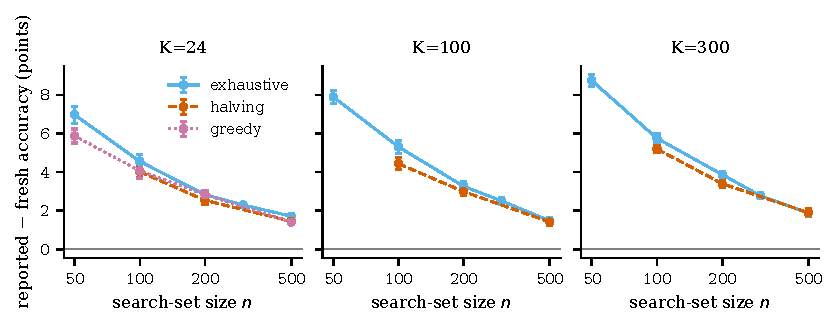
\includegraphics[width=\linewidth]{fig_b_t1.pdf}
\caption{\textbf{Search procedure (T1).} Optimism by exhaustive, successive-halving and greedy search (greedy only at $K=24$); panels $K=24,100,300$; $\pm1.96$ block SE.}
\label{fig:B1}
\end{figure}
\begin{figure}[h]
\centering
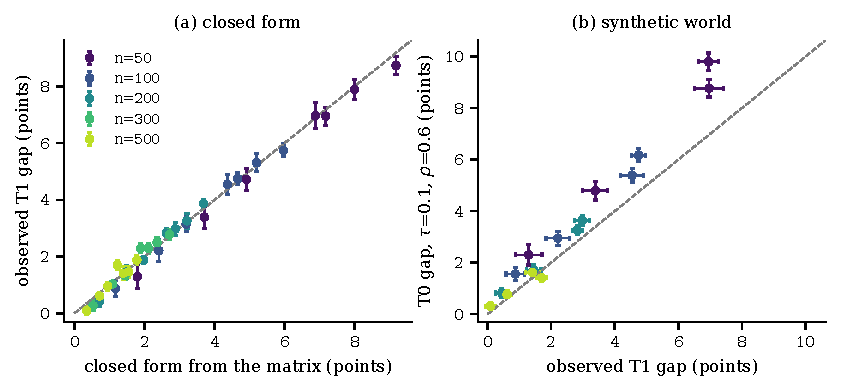
\includegraphics[width=\linewidth]{fig_t1_check.pdf}
\caption{\textbf{Checks of the extreme-value form and of the synthetic world against the real matrix (T1).} (a) Observed gap against the closed form fed with the matrix's $(\sigma,r,\tau)$, all 35 exhaustive cells. (b) Observed T1 gap against the T0 cells with the same $(n,K)$ at $\tau=0.1$, $\rho=0.6$ and baseline accuracy 0.3 (T0 is not calibrated to the matrix); dashed: $y=x$.}
\label{fig:T1check}
\end{figure}
\begin{figure}[h]
\centering
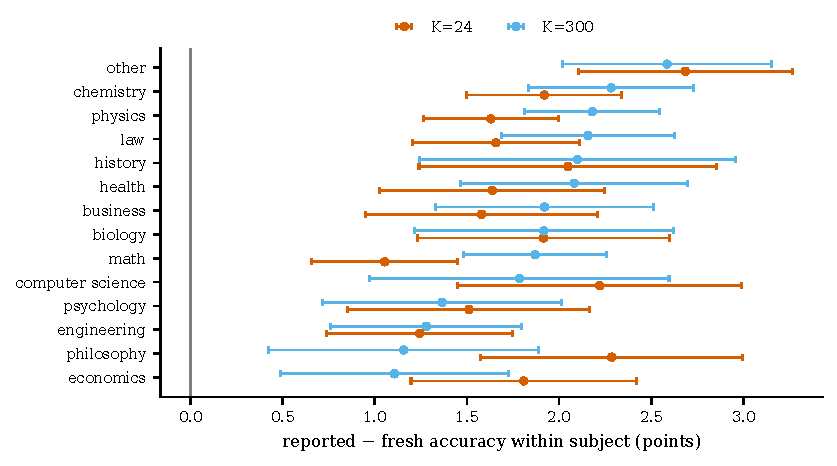
\includegraphics[width=\linewidth]{fig_t1_subjects.pdf}
\caption{\textbf{Gap by MMLU-Pro subject (T1)}, $n=500$, $K=24$ and $300$. A subject holds 16--63 of the 500 search items and replicates share items, so the bars understate uncertainty; the figure shows that optimism is present in every subject, not differences between subjects.}
\label{fig:T1subj}
\end{figure}

\section*{NeurIPS Paper Checklist}




\begin{enumerate}

\item {\bf Claims}
    \item[] Question: Do the main claims made in the abstract and introduction accurately reflect the paper's contributions and scope?
    \item[] Answer: \answerYes{}
    \item[] Justification: Abstract and Sec.~\ref{sec:intro} state the measured optimism, the decision consequences and the scope limits (one small model, replay not live search, no live tool run); Sec.~\ref{sec:discussion} lists them.
    \item[] Guidelines:
    \begin{itemize}
        \item The answer \answerNA{} means that the abstract and introduction do not include the claims made in the paper.
        \item The abstract and/or introduction should clearly state the claims made, including the contributions made in the paper and important assumptions and limitations. A \answerNo{} or \answerNA{} answer to this question will not be perceived well by the reviewers. 
        \item The claims made should match theoretical and experimental results, and reflect how much the results can be expected to generalize to other settings. 
        \item It is fine to include aspirational goals as motivation as long as it is clear that these goals are not attained by the paper. 
    \end{itemize}

\item {\bf Limitations}
    \item[] Question: Does the paper discuss the limitations of the work performed by the authors?
    \item[] Answer: \answerYes{}
    \item[] Justification: Sec.~\ref{sec:discussion} (Limitations i--ix) covers model scale, candidate family, replay versus live search, fixed pool, T0 calibration, heuristic formula, M4 only for exhaustive search, and compute.
    \item[] Guidelines:
    \begin{itemize}
        \item The answer \answerNA{} means that the paper has no limitation while the answer \answerNo{} means that the paper has limitations, but those are not discussed in the paper. 
        \item The authors are encouraged to create a separate ``Limitations'' section in their paper.
        \item The paper should point out any strong assumptions and how robust the results are to violations of these assumptions (e.g., independence assumptions, noiseless settings, model well-specification, asymptotic approximations only holding locally). The authors should reflect on how these assumptions might be violated in practice and what the implications would be.
        \item The authors should reflect on the scope of the claims made, e.g., if the approach was only tested on a few datasets or with a few runs. In general, empirical results often depend on implicit assumptions, which should be articulated.
        \item The authors should reflect on the factors that influence the performance of the approach. For example, a facial recognition algorithm may perform poorly when image resolution is low or images are taken in low lighting. Or a speech-to-text system might not be used reliably to provide closed captions for online lectures because it fails to handle technical jargon.
        \item The authors should discuss the computational efficiency of the proposed algorithms and how they scale with dataset size.
        \item If applicable, the authors should discuss possible limitations of their approach to address problems of privacy and fairness.
        \item While the authors might fear that complete honesty about limitations might be used by reviewers as grounds for rejection, a worse outcome might be that reviewers discover limitations that aren't acknowledged in the paper. The authors should use their best judgment and recognize that individual actions in favor of transparency play an important role in developing norms that preserve the integrity of the community. Reviewers will be specifically instructed to not penalize honesty concerning limitations.
    \end{itemize}

\item {\bf Theory assumptions and proofs}
    \item[] Question: For each theoretical result, does the paper provide the full set of assumptions and a complete (and correct) proof?
    \item[] Answer: \answerNA{}
    \item[] Justification: The paper has no theorems; the extreme-value formula in Sec.~\ref{sec:method} is a stated heuristic approximation that is checked numerically, not proved.
    \item[] Guidelines:
    \begin{itemize}
        \item The answer \answerNA{} means that the paper does not include theoretical results. 
        \item All the theorems, formulas, and proofs in the paper should be numbered and cross-referenced.
        \item All assumptions should be clearly stated or referenced in the statement of any theorems.
        \item The proofs can either appear in the main paper or the supplemental material, but if they appear in the supplemental material, the authors are encouraged to provide a short proof sketch to provide intuition. 
        \item Inversely, any informal proof provided in the core of the paper should be complemented by formal proofs provided in appendix or supplemental material.
        \item Theorems and Lemmas that the proof relies upon should be properly referenced. 
    \end{itemize}

    \item {\bf Experimental result reproducibility}
    \item[] Question: Does the paper fully disclose all the information needed to reproduce the main experimental results of the paper to the extent that it affects the main claims and/or conclusions of the paper (regardless of whether the code and data are provided or not)?
    \item[] Answer: \answerYes{}
    \item[] Justification: Sec.~\ref{sec:method}, Sec.~\ref{sec:experiments} and the appendix define the setting, estimands, methods M0--M5, grids, seeds, models, dataset revision and replicate counts; \texttt{REPRODUCE.md} gives the commands.
    \item[] Guidelines:
    \begin{itemize}
        \item The answer \answerNA{} means that the paper does not include experiments.
        \item If the paper includes experiments, a \answerNo{} answer to this question will not be perceived well by the reviewers: Making the paper reproducible is important, regardless of whether the code and data are provided or not.
        \item If the contribution is a dataset and\slash or model, the authors should describe the steps taken to make their results reproducible or verifiable. 
        \item Depending on the contribution, reproducibility can be accomplished in various ways. For example, if the contribution is a novel architecture, describing the architecture fully might suffice, or if the contribution is a specific model and empirical evaluation, it may be necessary to either make it possible for others to replicate the model with the same dataset, or provide access to the model. In general. releasing code and data is often one good way to accomplish this, but reproducibility can also be provided via detailed instructions for how to replicate the results, access to a hosted model (e.g., in the case of a large language model), releasing of a model checkpoint, or other means that are appropriate to the research performed.
        \item While NeurIPS does not require releasing code, the conference does require all submissions to provide some reasonable avenue for reproducibility, which may depend on the nature of the contribution. For example
        \begin{enumerate}
            \item If the contribution is primarily a new algorithm, the paper should make it clear how to reproduce that algorithm.
            \item If the contribution is primarily a new model architecture, the paper should describe the architecture clearly and fully.
            \item If the contribution is a new model (e.g., a large language model), then there should either be a way to access this model for reproducing the results or a way to reproduce the model (e.g., with an open-source dataset or instructions for how to construct the dataset).
            \item We recognize that reproducibility may be tricky in some cases, in which case authors are welcome to describe the particular way they provide for reproducibility. In the case of closed-source models, it may be that access to the model is limited in some way (e.g., to registered users), but it should be possible for other researchers to have some path to reproducing or verifying the results.
        \end{enumerate}
    \end{itemize}


\item {\bf Open access to data and code}
    \item[] Question: Does the paper provide open access to the data and code, with sufficient instructions to faithfully reproduce the main experimental results, as described in supplemental material?
    \item[] Answer: \answerYes{}
    \item[] Justification: Code, per-item outcome matrices and result files are in the anonymous repository delivered with the paper; \texttt{REPRODUCE.md} lists the commands and the pinned MMLU-Pro revision and model file (public assets).
    \item[] Guidelines:
    \begin{itemize}
        \item The answer \answerNA{} means that paper does not include experiments requiring code.
        \item Please see the NeurIPS code and data submission guidelines (\url{https://neurips.cc/public/guides/CodeSubmissionPolicy}) for more details.
        \item While we encourage the release of code and data, we understand that this might not be possible, so \answerNo{} is an acceptable answer. Papers cannot be rejected simply for not including code, unless this is central to the contribution (e.g., for a new open-source benchmark).
        \item The instructions should contain the exact command and environment needed to run to reproduce the results. See the NeurIPS code and data submission guidelines (\url{https://neurips.cc/public/guides/CodeSubmissionPolicy}) for more details.
        \item The authors should provide instructions on data access and preparation, including how to access the raw data, preprocessed data, intermediate data, and generated data, etc.
        \item The authors should provide scripts to reproduce all experimental results for the new proposed method and baselines. If only a subset of experiments are reproducible, they should state which ones are omitted from the script and why.
        \item At submission time, to preserve anonymity, the authors should release anonymized versions (if applicable).
        \item Providing as much information as possible in supplemental material (appended to the paper) is recommended, but including URLs to data and code is permitted.
    \end{itemize}


\item {\bf Experimental setting/details}
    \item[] Question: Does the paper specify all the training and test details (e.g., data splits, hyperparameters, how they were chosen, type of optimizer) necessary to understand the results?
    \item[] Answer: \answerYes{}
    \item[] Justification: Sec.~\ref{sec:experiments} and Sec.~\ref{sec:t1} give the search-set and fresh-set construction, grids of $n$, $K$ and $\tau$, search procedures and the fixed configuration family; nothing is trained, and no hyperparameter was tuned on the fresh items.
    \item[] Guidelines:
    \begin{itemize}
        \item The answer \answerNA{} means that the paper does not include experiments.
        \item The experimental setting should be presented in the core of the paper to a level of detail that is necessary to appreciate the results and make sense of them.
        \item The full details can be provided either with the code, in appendix, or as supplemental material.
    \end{itemize}

\item {\bf Experiment statistical significance}
    \item[] Question: Does the paper report error bars suitably and correctly defined or other appropriate information about the statistical significance of the experiments?
    \item[] Answer: \answerYes{}
    \item[] Justification: Intervals are mean$\pm1.96$ SE over replicates and Wilson 95\% intervals in the synthetic world (T0) and $\pm1.96$ delete-a-block SEs on the real matrix (T1), where replicates share one pool (Sec.~\ref{sec:t1}, Limitation iv).
    \item[] Guidelines:
    \begin{itemize}
        \item The answer \answerNA{} means that the paper does not include experiments.
        \item The authors should answer \answerYes{} if the results are accompanied by error bars, confidence intervals, or statistical significance tests, at least for the experiments that support the main claims of the paper.
        \item The factors of variability that the error bars are capturing should be clearly stated (for example, train/test split, initialization, random drawing of some parameter, or overall run with given experimental conditions).
        \item The method for calculating the error bars should be explained (closed form formula, call to a library function, bootstrap, etc.)
        \item The assumptions made should be given (e.g., Normally distributed errors).
        \item It should be clear whether the error bar is the standard deviation or the standard error of the mean.
        \item It is OK to report 1-sigma error bars, but one should state it. The authors should preferably report a 2-sigma error bar than state that they have a 96\% CI, if the hypothesis of Normality of errors is not verified.
        \item For asymmetric distributions, the authors should be careful not to show in tables or figures symmetric error bars that would yield results that are out of range (e.g., negative error rates).
        \item If error bars are reported in tables or plots, the authors should explain in the text how they were calculated and reference the corresponding figures or tables in the text.
    \end{itemize}

\item {\bf Experiments compute resources}
    \item[] Question: For each experiment, does the paper provide sufficient information on the computer resources (type of compute workers, memory, time of execution) needed to reproduce the experiments?
    \item[] Answer: \answerYes{}
    \item[] Justification: Appendix Table~\ref{tab:F} and Limitation (ix) give wall times, hardware (2-vCPU CPU containers, no GPU) and call counts for every job.
    \item[] Guidelines:
    \begin{itemize}
        \item The answer \answerNA{} means that the paper does not include experiments.
        \item The paper should indicate the type of compute workers CPU or GPU, internal cluster, or cloud provider, including relevant memory and storage.
        \item The paper should provide the amount of compute required for each of the individual experimental runs as well as estimate the total compute. 
        \item The paper should disclose whether the full research project required more compute than the experiments reported in the paper (e.g., preliminary or failed experiments that didn't make it into the paper). 
    \end{itemize}
    
\item {\bf Code of ethics}
    \item[] Question: Does the research conducted in the paper conform, in every respect, with the NeurIPS Code of Ethics \url{https://neurips.cc/public/EthicsGuidelines}?
    \item[] Answer: \answerYes{}
    \item[] Justification: The work uses synthetic data and public benchmark items with a public model; no human subjects, no personal data, and no deviation from the Code of Ethics that we are aware of.
    \item[] Guidelines:
    \begin{itemize}
        \item The answer \answerNA{} means that the authors have not reviewed the NeurIPS Code of Ethics.
        \item If the authors answer \answerNo, they should explain the special circumstances that require a deviation from the Code of Ethics.
        \item The authors should make sure to preserve anonymity (e.g., if there is a special consideration due to laws or regulations in their jurisdiction).
    \end{itemize}


\item {\bf Broader impacts}
    \item[] Question: Does the paper discuss both potential positive societal impacts and negative societal impacts of the work performed?
    \item[] Answer: \answerNA{}
    \item[] Justification: This is a methodological study of how reported benchmark scores of tuned systems should be read; we see no direct societal impact beyond better evaluation practice, and the Discussion notes that over-optimistic reports can mislead readers about system quality.
    \item[] Guidelines:
    \begin{itemize}
        \item The answer \answerNA{} means that there is no societal impact of the work performed.
        \item If the authors answer \answerNA{} or \answerNo, they should explain why their work has no societal impact or why the paper does not address societal impact.
        \item Examples of negative societal impacts include potential malicious or unintended uses (e.g., disinformation, generating fake profiles, surveillance), fairness considerations (e.g., deployment of technologies that could make decisions that unfairly impact specific groups), privacy considerations, and security considerations.
        \item The conference expects that many papers will be foundational research and not tied to particular applications, let alone deployments. However, if there is a direct path to any negative applications, the authors should point it out. For example, it is legitimate to point out that an improvement in the quality of generative models could be used to generate Deepfakes for disinformation. On the other hand, it is not needed to point out that a generic algorithm for optimizing neural networks could enable people to train models that generate Deepfakes faster.
        \item The authors should consider possible harms that could arise when the technology is being used as intended and functioning correctly, harms that could arise when the technology is being used as intended but gives incorrect results, and harms following from (intentional or unintentional) misuse of the technology.
        \item If there are negative societal impacts, the authors could also discuss possible mitigation strategies (e.g., gated release of models, providing defenses in addition to attacks, mechanisms for monitoring misuse, mechanisms to monitor how a system learns from feedback over time, improving the efficiency and accessibility of ML).
    \end{itemize}
    
\item {\bf Safeguards}
    \item[] Question: Does the paper describe safeguards that have been put in place for responsible release of data or models that have a high risk for misuse (e.g., pre-trained language models, image generators, or scraped datasets)?
    \item[] Answer: \answerNA{}
    \item[] Justification: We release simulation code and score matrices of a small public model on a public benchmark; there is no high-risk model or scraped data.
    \item[] Guidelines:
    \begin{itemize}
        \item The answer \answerNA{} means that the paper poses no such risks.
        \item Released models that have a high risk for misuse or dual-use should be released with necessary safeguards to allow for controlled use of the model, for example by requiring that users adhere to usage guidelines or restrictions to access the model or implementing safety filters. 
        \item Datasets that have been scraped from the Internet could pose safety risks. The authors should describe how they avoided releasing unsafe images.
        \item We recognize that providing effective safeguards is challenging, and many papers do not require this, but we encourage authors to take this into account and make a best faith effort.
    \end{itemize}

\item {\bf Licenses for existing assets}
    \item[] Question: Are the creators or original owners of assets (e.g., code, data, models), used in the paper, properly credited and are the license and terms of use explicitly mentioned and properly respected?
    \item[] Answer: \answerYes{}
    \item[] Justification: MMLU-Pro~\citep{wang2024mmlupro} (MIT license), Qwen2.5-1.5B-Instruct~\citep{qwen2024qwen25} (Apache-2.0) and llama.cpp (MIT) are cited or named with their versions and licenses in Sec.~\ref{sec:t1} and \texttt{REPRODUCE.md}.
    \item[] Guidelines:
    \begin{itemize}
        \item The answer \answerNA{} means that the paper does not use existing assets.
        \item The authors should cite the original paper that produced the code package or dataset.
        \item The authors should state which version of the asset is used and, if possible, include a URL.
        \item The name of the license (e.g., CC-BY 4.0) should be included for each asset.
        \item For scraped data from a particular source (e.g., website), the copyright and terms of service of that source should be provided.
        \item If assets are released, the license, copyright information, and terms of use in the package should be provided. For popular datasets, \url{paperswithcode.com/datasets} has curated licenses for some datasets. Their licensing guide can help determine the license of a dataset.
        \item For existing datasets that are re-packaged, both the original license and the license of the derived asset (if it has changed) should be provided.
        \item If this information is not available online, the authors are encouraged to reach out to the asset's creators.
    \end{itemize}

\item {\bf New assets}
    \item[] Question: Are new assets introduced in the paper well documented and is the documentation provided alongside the assets?
    \item[] Answer: \answerYes{}
    \item[] Justification: The released code, result schema (\texttt{results/SCHEMA.md}) and manifest document the new simulation, replay code and cached outcome matrices; \texttt{REPRODUCE.md} explains how to regenerate them.
    \item[] Guidelines:
    \begin{itemize}
        \item The answer \answerNA{} means that the paper does not release new assets.
        \item Researchers should communicate the details of the dataset\slash code\slash model as part of their submissions via structured templates. This includes details about training, license, limitations, etc. 
        \item The paper should discuss whether and how consent was obtained from people whose asset is used.
        \item At submission time, remember to anonymize your assets (if applicable). You can either create an anonymized URL or include an anonymized zip file.
    \end{itemize}

\item {\bf Crowdsourcing and research with human subjects}
    \item[] Question: For crowdsourcing experiments and research with human subjects, does the paper include the full text of instructions given to participants and screenshots, if applicable, as well as details about compensation (if any)? 
    \item[] Answer: \answerNA{}
    \item[] Justification: No crowdsourcing or human-subject research.
    \item[] Guidelines:
    \begin{itemize}
        \item The answer \answerNA{} means that the paper does not involve crowdsourcing nor research with human subjects.
        \item Including this information in the supplemental material is fine, but if the main contribution of the paper involves human subjects, then as much detail as possible should be included in the main paper. 
        \item According to the NeurIPS Code of Ethics, workers involved in data collection, curation, or other labor should be paid at least the minimum wage in the country of the data collector. 
    \end{itemize}

\item {\bf Institutional review board (IRB) approvals or equivalent for research with human subjects}
    \item[] Question: Does the paper describe potential risks incurred by study participants, whether such risks were disclosed to the subjects, and whether Institutional Review Board (IRB) approvals (or an equivalent approval/review based on the requirements of your country or institution) were obtained?
    \item[] Answer: \answerNA{}
    \item[] Justification: No human subjects, so no IRB approval was needed.
    \item[] Guidelines:
    \begin{itemize}
        \item The answer \answerNA{} means that the paper does not involve crowdsourcing nor research with human subjects.
        \item Depending on the country in which research is conducted, IRB approval (or equivalent) may be required for any human subjects research. If you obtained IRB approval, you should clearly state this in the paper. 
        \item We recognize that the procedures for this may vary significantly between institutions and locations, and we expect authors to adhere to the NeurIPS Code of Ethics and the guidelines for their institution. 
        \item For initial submissions, do not include any information that would break anonymity (if applicable), such as the institution conducting the review.
    \end{itemize}

\item {\bf Declaration of LLM usage}
    \item[] Question: Does the paper describe the usage of LLMs if it is an important, original, or non-standard component of the core methods in this research? Note that if the LLM is used only for writing, editing, or formatting purposes and does \emph{not} impact the core methodology, scientific rigor, or originality of the research, declaration is not required.
    %this research? 
    \item[] Answer: \answerYes{}
    \item[] Justification: An LLM (Qwen2.5-1.5B-Instruct, run locally) is the system whose outputs are studied; its use, prompts and scoring are described in Sec.~\ref{sec:t1}. The manuscript was drafted with an AI assistant, which does not affect the methodology.
    \item[] Guidelines:
    \begin{itemize}
        \item The answer \answerNA{} means that the core method development in this research does not involve LLMs as any important, original, or non-standard components.
        \item Please refer to our LLM policy in the NeurIPS handbook for what should or should not be described.
    \end{itemize}

\end{enumerate}
\end{document}
